\section{Материал и методика}
	\subsection{География исследований}

		\subsubsection{Белое море}
В вершине Кандалакшского залива наблюдения проводили на $6$ участках в рамках работы экспедиций Группы исследований прибрежных сообществ Лаборатории экологии морского бентоса (гидробиологии) СПбГДТЮ (рис.~\ref{ris:karta_Kandalaksha}). 
    \begin{figure}
    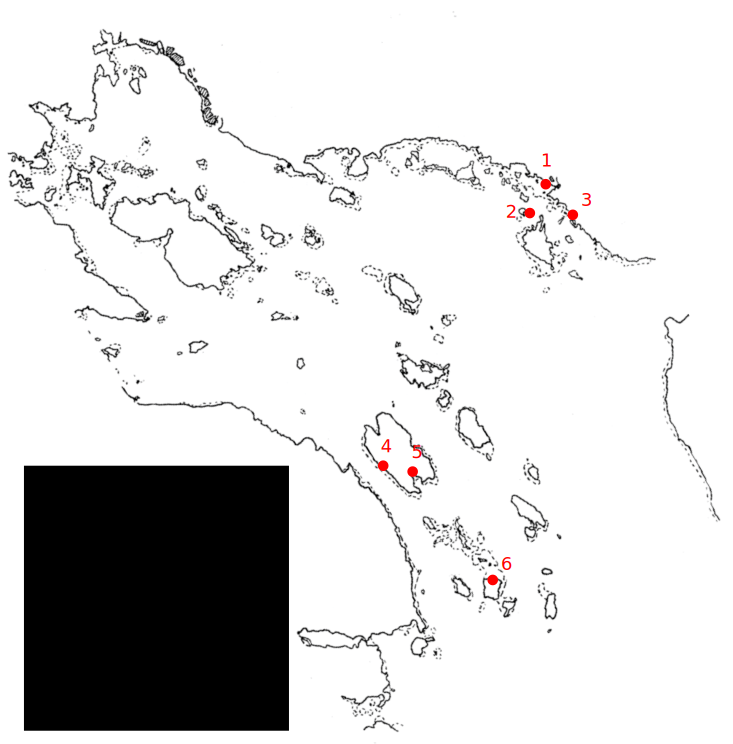
\includegraphics[width=\textwidth]{../maps/map_Kandalaksha.pdf}
    \caption{Исследованные участки в вершине Кандалакшского залива Белого моря}
    \label{ris:karta_Kandalaksha}
    \end{figure}
Три участка расположены в районе Лувеньгских шхер: эстуарий реки Лувеньги, Илистая губа острова Горелого и участок материковой литорали в $800$ метрах западнее поселка Лувеньга.
Один участок был расположен на литорали острова Ряшков в Западной Ряшковой салме (Северный архипелаг).
В работе использованы данные Д.\:А.~Аристова из Южной губы о.~Ряшков и с о.~Большой Ломнишный (Северный архипелаг) (рис.~\ref{ris:karta_Kandalaksha}). 

В районе губы Чупа исследования проводили на $4$ участках (рис.~\ref{ris:karta_Chupa}) в ходе экспедиций кафедры ихтиологии и гидробиологии СПбГУ. 
\begin{figure}
    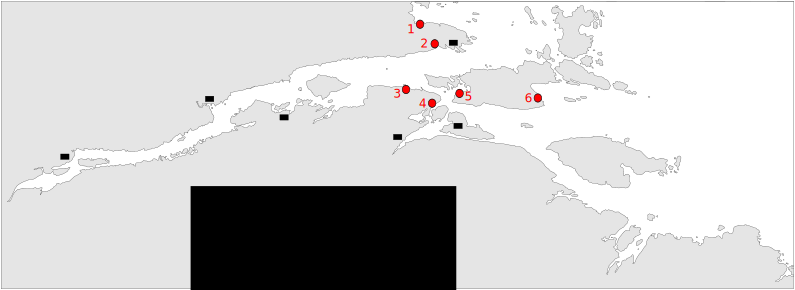
\includegraphics[width=\textwidth]{../maps/map_Chupa.pdf}
    \caption{Исследованные участки в районе губы Чупа Белого моря}
    \label{ris:karta_Chupa}
\end{figure}
Два участка были расположены на литорали острова Кереть --- в Сухой салме и бухте Клющиха. 
Один участок был расположен на материковой литорали пролива Подпахта и один --- в бухте Лисьей.

Также в работе использованы данные ББС <<Картеш>> ЗИН РАН по обилию маком в губах Медвежья и Сельдяная (\cite{Varfolomeeva_Naumov_2013}) (рис.~\ref{ris:karta_Chupa}).

		\subsubsection{Баренцево море}
Материал  в акватории Баренцева моря  был  собран    в ходе   студенческой баренцевоморской экспедиции СПбГУ. 
Всего было исследовано $8$ участков --- $2$ в Кольском заливе (рис.~\ref{ris:karta_Kolskiy})   и   $6$  в   прибрежной   зоне  Восточного  Мурмана (рис.~\ref{ris:karta_Murman}).  
Участки литорали  в   Кольском   заливе   были  расположены на побережье в районе Абрам-мыса и в Палa-губе, в районе города Полярный. 
На   Восточном   Мурмане исследованные участки литорали  были   расположены   в   губах   Гавриловская,  Ярнышная, Дальнезеленецкая, Шельпинская, Порчниха и Ивановская.

Также в работе использованы данные К.\:В.~Шунькиной и Е.\:А.~Генельт-Яновского по обилию маком в губе Печенга (Западный Мурман) (рис.~\ref{ris:karta_Murman}), и в районе Северного Нагорного и Ретинского (Кольский залив) (рис.~\ref{ris:karta_Kolskiy}).

    \subsection{Характеристика местообитаний}
Для всех участков было составлено физиономическое описание.

Удобной комплексной оценкой гидродинамики региона и условий питания детритофагов служат показатели состава грунта. 
Поэтому на ряде исследованных участков были отобраны образцы грунта. 
В экспедиции после отбора из грунта выбирали крупных животных (червей, раков, моллюсков, приапулид), образцы высушивали и упаковывали для отправки в город. 
В городе образцы досушивали в термостате при температуре $105^o$C до момента, когда масса образца переставала изменяться. 
Из каждого образца брали по три навески грунта для определения содержания органических веществ. 
Навески помещали в муфельную печь с температурой $450^o$C на $8$ часов. 
После сжигания навески повторно взвешивали, и по разнице масс определяли массовую долю органических веществ в грунте. 
По трем навескам рассчитывали среднюю массовую долю для каждого образца.

Оставшийся грунт использовали для определения гранулометрического состава. 
Для этого грунт взвешивали, после чего просеивали в сухом состоянии через колонку сит (диаметр ячеи: $10 - 5 - 3 - 1 - 0,5 - 0,25$~мм). 
Частицы размером менее $0,25$~мм просеивали через сито с диаметром ячеи $0,1$~мм с использованием струи воды, после чего оставшиеся на сите --- высушивали при температуре $105^o$C. 
Каждую фракцию частиц взвешивали, и определяли их массовую долю. 
Поскольку доля частиц размером менее $0,1$~мм составила менее 5\% во всех образцах, то дальнейшее разделение этой фракции по размеру не проводили. 
При описании гранулометрического состава грунта использовали классификацию И.\,Л.~Безрукова и А.\,Н.,~Лисицина для морских водоемов (таблица~\ref{tab:lisicyn_granulometriya}, \cite{Bezrukov_Lisicyn_1960}).
\begin{table}[h]
    \centering
    \caption{Классификация фракций грунта по размеру частиц (\cite{Bezrukov_Lisicyn_1960})}
    \label{tab:lisicyn_granulometriya}
\begin{tabular}{|l|l|}
    \hline
    Размер фракции,~мм & Название фракции         \\ \hline
     $> 10$    & Крупный и средний гравий  \\
    $10-5$               & Мелкий гравий         \\
    $5-3$                & Очень мелкий гравий   \\
    $3-1$                & Очень крупный песок   \\
    $1-0,5$              & Крупный песок         \\
    $0,5-0,25$           & Средний песок         \\
    $0,25-0,1$           & Мелкий песок          \\
    $0,1-0,05$           & Крупный алеврит       \\
    $0,05-0,01$          & Средний алеврит       \\
    $0,01-0,005$         & Мелкий алеврит        \\
    $< 0,005$     & Пелит                   \\ \hline
\end{tabular}
\end{table}

    \subsection{Описание сообществ, включающих {\it Macoma balthica}}
\textcolor{red}{А что тут про Беломорских?..}

На каждом участке в акватории Баренцева моря исследовали все  горизонты литорали, представленные мягкими грунтами.  
На каждом горизонте отбирали от $5$ до $87$ проб  (табл.  \ref{tab:}). Таким образом, всего было составлено $16$ описаний.

Как основное орудие сбора использовали литоральную рамку площадью $1/30$~м$^2$, из которой изымали грунт на глубину $5$~см. 
В случае, когда приходилось отбирать пробы из-под воды, использовали зубчатый водолазный дночерпатель площадью захвата $1/20$~м$^2$.
Отобранные пробы промывали на сите с диаметром ячеи $1$~мм. 
После промывки из   проб   выбирали   всех   особей  {\it Macoma   balthica}  и   представителей   сопутствующего макрозообентоса    для   определения   состава   сообщества.
Представителей   сопутствующего макрозообентоса  определяли   до   минимально   возможного   таксона.

Для сравнения видового состава сообщества использовали коэффициент Жаккара. 
Результаты визуализировали при помощи  кластерного анализа методом ближайшего соседа. 
Для оценки влияния факторов использовали многомерное шкалирование MDS в сочетании с анализом сходства ANOSIM.
Анализы проводили в программе PaSt (\cite{Hammer_et_al_2001}).


	\subsection{Изучение микрораспределения {\it Macoma balthica}}

\textcolor{red}{квадраты на Белом}

\textcolor{red}{квадраты на Баренцевом}
При оценке распределения особей в губе Порчниха в 2007 г. было отобрано 32 пробы рамкой 1/30м2, причем пробы брались вплотную друг к другу 4 рядами по 8 шт.

% из Генельт-Кобылков-Назарова, 2007 (что это было??)
Вторая схема изучения распределения особей {\it Macoma baltica} была проведена по методике, описанной Трашем (\cite{Thrush_et_al_1989}) с изменением масштаба.
Исследования были проведены в августе $2007$~г. на илисто-песчаной литорали кутовых участков губ Восточного Мурмана --- Ярнышной и Дальнезеленецкой, и в октябре $2007$~г. на литорали Пала-губы (Кольский залив). 
Для Дальнезеленецкой губы съемка была повторена в августе $2008$ года двукратно.

В каждой точке отбиралось по $36$ проб площадью $1/30$~м$^2$, расположенных в пределах участка размером $7,5 \times 12$~м. 
Координаты каждой пробы были определены в декартовой системе координат в метрах, один из углов участка служил точкой отсчета. 
В дальнейшем пробы промывали на сите с диаметром ячеи $1$~мм. 
В лаборатории были выбраны и  подсчитаны все моллюски, ракообразные и приапулиды.

При дальнейшей обработке данных для каждого участках подсчитывали индекс структурности (отношение дисперсии к средней арифметической). 
Для анализа размеров агрегаций были построены коррелограммы, основанные на коэффициенте пространственной автокорреляции Морана (\cite{ncf}).
Достоверность коэффициентов определяли пермутационным методом.
Наличие градиентов определяли с использованием корреляционного анализа Кенделла между координатами проб и обилием вида в каждой пробе. 
Все статистические анализы проводили в статистической среде \R{} (\cite{R_2014}) с $95\%$ доверительной вероятностью ($P < 0,05$).



	
	\subsection{Изучение структуры поселений {\it Macoma balthica}}
Изучение размерной структуры поселений маком проводили на всех участках.
Для этого у всех моллюсков в пробах под бинокуляром измеряли максимальный линейный размер (длину) с точностью $0,1$~мм.

  На каждом участке в акватории Баренцева моря исследовали все  горизонты литорали, представленные мягкими грунтами.  
На каждом горизонте отбирали от $5$ до $87$ проб  (табл.  \ref{tab:}). Всего было составлено $16$ описаний.

Как основное орудие сбора использовали литоральную рамку площадью $1/30$~м$^2$, из которой изымали грунт на глубину $5$~см. 
В случае, когда приходилось отбирать пробы из-под воды, использовали зубчатый водолазный дночерпатель площадью захвата $1/20$~м2.
Отобранные пробы промывали на сите с диаметром ячеи $1$~мм. 
После промывки из   проб   выбирали   всех   особей  {\it Macoma balthica}.

   Маком   измеряли  с точностью $0,1$~мм  и взвешивали с точностью $10$~мг.
 У всех особей измеряли максимальный линейный размер (длину). 
В дальнейшем по этим данным строили графики размерной структуры поселений. 

Кроме того, у моллюсков подсчитывали количество меток зимней остановки роста, которое принимали как возраст моллюсков --- число прожитых зим (например, $4+$ это  особи возрастом от $4$ до $5$ лет).   
Таким   образом   были   получены   оценки возрастной структуры поселений {\it M. balthica}.

	\subsection{Изучение динамики поселений {\it Macoma balthica}}
        \subsubsection{Белое море}
В Белом море динамику поселений {\it Macoma balthica} исследовали на $6$ участках в районе вершины Кандалакшского залива. 

Сборы проводили с 1992 по 2012 год ежегодно в июле-августе.
Автор принимала участие в полевых сборах с $1999$ по $2007$ год.
Данные за другие годы взяты из архива ГИПС ЛЭМБ.

Структура материала представлена в таблице \ref{tab:material_Kandalaksha}.
\begin{table}
%\begin{tabular}{|*{5}{p{0.2\textwidth}|}} \hline
    \begin{tabularx}{\textwidth}{|*{5}{X|}} \hline
участок & годы наблюдения & обследованные горизонты литорали & количество проб в однократной съемке & площадь пробоотборника  \\ \hline
о. Горелый Лувеньгских шхер & 1992 -- 2012 & ВГЛ, СГЛ, НГЛ & 1-3 & 1/30, 1/10 \\ \hline
Материковая литораль в районе пос. Лувеньга & 1992-2000, 2002, 2004 & ВГЛ, СГЛ, НГЛ & 12-20 & 1/30 \\ \hline
Эстуарий р. Лувеньги & 1992 -- 2012 & СГЛ & 3 & 1/10 \\ \hline
Литораль Западной Ряшковой салмы о. Ряшкова & 1994 -- 2012 & СГЛ & 2 & 1/10 \\ \hline
Южная губа о. Ряшкова & 2001 -- 2012 & НГЛ & 9-16 & 1/30 \\ \hline
о. Ломнишный & 2007 -- 2012 & НГЛ & 5-10 & 1/30  \\ \hline
\end{tabularx}
\caption{Структура материала по динамике поселений{\it Macoma balthica} вершины Кандалакшского залива}
\label{tab:material_Kandalaksha}
\end{table}

На каждом исследованном участке отбирали $3 - 25$ проб площадью $1/30 - 1/10$~м$^2$, которые затем промывали на сите с диаметром ячеи $0,5 - 1$~мм. 
В пробах учитывали всех особей {\it Macoma balthica}, у которых в дальнейшем измеряли максимальный линейный размер (длину) с точностью ~0,1~мм. 

Для определения биомассы моллюсков взвешивали на электронных весах с точностью до $1$~мг. 
Для серий проб, где не проводили взвешивание моллюсков, биомассу определяли рассчетным методом с использованием аллометриеской зависимости сырой массы маком от длины их раковины \cite{Maximovich_et_al_1993}.

В дальнейшем рассчитывали показатели средней численности маком на квадратный метр (плотность поселения) и размерно-частотное распределение особоей.
Для построения размерно-частотного распределения шаг размерного класса составлял $1$~мм.

В дальнейшем при анализе мы работали с особями с длиной раковины более $1,0$~мм по двум причинам. 
Во-первых, для того чтобы сделать сравнимыми результаты с разных участков, где пробы промывались на ситах с разным диаметром ячеи. 
Во-вторых, пробы отбирали в середине лета, то есть к этому моменту молодь этого года частично осела, то есть оценка численности данной группы будет некорректна.
Мы считаем корректной такую редукцию материала, поскольку для Белого моря показано, что усешность пополнения поселений молодью в первую очередь зависит от выживаемости спата зимой (\textcolor{red}{тут ссылка на каких-то Максимовича-Герасимову. 2004 - БиНИИ? или 2012 - Hydrobiology}).

Для анализа динамики пополнения поселений молодью в $2012 - 2013$ годах у особей длиной менее $3$~мм были измерены длины колец зимней остановки роста. 
После определения размеров годовалых особей, по размерной было рассчитано их обилие в каждом году мониторингового наблюдения.
Всего было промерено \textcolor{red}{проверить, сколько промерено} 496 особей.



В работе использованы мониторинговые данные кафедры ихтиологии и гидробиологии СПбГУ по обоим участкам на острове Кереть (\cite{Maximovich_et_al_1991, Gerasimova_Maximovich_2013}) (рис.~\ref{ris:karta_Chupa}). 
Также в работе использованы многолетие данные ББС <<Картеш>> ЗИН РАН по обилию маком в губах Медвежья и Сельдяная (\cite{Varfolomeeva_Naumov_2013}) (рис.~\ref{ris:karta_Chupa}).


 
%методика из Назаровой-Полоскина
%Материал собран в августе 1992 - 2003 гг. Изучено три литоральных поселения маком: в Илистой губе острова Горелого (участок 1), в эстуарии реки Лувеньги (участок 2) и на материковой литорали к югу от поселка Лувеньга (участок 3). Сборы проведены пробоотборником площадью захвата 1/30 м2. Разовая выборка составляла от 9 до 25 проб с участка. Грунт выбирался до глубины 5 см и промывался на сите с диаметром ячеи 0.5мм.  Всех особей  M. balthica измеряли с точностью 0.1 мм. В каждый момент наблюдений определяли размерную структуру и плотность поселения маком. 



% методика из Аристова
%Оба участка закрыты от волнового воздейст-
%вия. Литораль в районе исследований представляет собой песчаный пляж с примесью
%ила с вкраплениями крупных валунов. Спуск в сублитораль пологий, отчетливо вы-
%раженный пояс фукоидов отсутствует. Население представлено типичными формами,
%такими как Arenicola marina, Macoma balthica, Mya arenaria, Hydrobia ulvae, Microspio sp.
%и др. (Д. А. Аристов, неопубликованные данные).
%В обеих точках производили сборы по следующей методике: в районе нуля глубин
%во время отлива в пределах участков случайным образом выбирали и обследовали не-
%сколько площадок. Поскольку радиусы индивидуальной активности A. islandica и пред-
%полагаемых жертв (двустворчатых моллюсков) существенно различаются, в пределах
%каждой площадки брали пару проб методом вложенных рамок. Первую пробу из пары
%(1/4 м2) брали для учета A. islandica. Грунт из пробы тщательно перебирали вручную,
%всех найденных представителей сем. Naticidae подсчитывали и определяли их видовую
%принадлежность. Вторая проба (1/30 м2) была взята для учета потенциальных жертв —
%двустворчатых моллюсков. Грунт из нее промывали на сите с диаметром ячеи 1 мм,
%а затем остаток разбирали в фотографической кювете с белым дном. Из грунта соби


        \subsection{Баренцево море}
% из Дерюгинских, 2007 + новой статьи

В Баренцевом море динамику поселений маком исследовали на модельном участке --- литоральной отмели Дальний пляж губы Дальнезеленецкой. 
В работе использованы материалы экспедиции по мониторингу Дальнего пляжа губы Дальнезеленецкой с $2002$ года, любезно предоставленные Е.\:А.~Генельт-Яновским.
Автор принимал участие в полевых сборах в $2006 - 2008$~гг.

Материал был собран в июле-августе $2002 - 2008$~гг. в пределах от верхнего горизонта песчаной литорали ($+2,0$~м) до $+0,7$~м над нулем глубин. 

 В $2002$ году была заложена сетка из $8$ станций (рис.~\ref{ris:karta_DP}). 
 В пределах каждой станции отбирали $3$ пирамиды рамок $1/245$ + $1/30$~м$^2$. 
 Пробы площадью $1/245$~м$^2$ промывали на сите с диаметром ячеи $0,5$~мм, внешние пробы площадью $1/30$~м$^2$ --- на сите с диаметром ячеи $1$~мм. 
 Для проб площадью $1/245$~м$^2$ проводили полную количественную разборку с последующей таксономический идентификацией особей и их подсчетом. 
 В пробах  площадью $1/30$~м$^2$ учитывали крупные виды Polychaeta и всех Bivalvia. 
 Также в районе каждой станции отбирали по $3--5$ проб площадью $1/10$~м$^2$, которые также промывали на сите с диаметром ячеи $1$~мм, для учета двустворчатых моллюсков.  
 У всех двустворчатых моллюсков измеряли длину раковины с точностью $0,1$~мм. 
 На каждой станции в $5$ рамках площадью $1/4$~м$^2$ проводился визуальный учет {\it Arenicola marina}.

 В $2003$ году съемка была повторена в полном объеме и введена $9$ станция, на которой отбирали только пробы для учета моллюсков (рис.~\ref{ris:karta_DP}). 
 В последующие годы отбирали пробы на трех станциях из $8$ (№$1-3$, рис.~\ref{ris:karta_DP}). 
 В $2008$ году отбирали пробы только для исследования двустворчатых моллюсков.

 В качестве точки сравнения нами был выбран $1973$ год (\cite{Streltsov_et_al_1974, Agarova_et_al_1976}), поскольку в тот год была проведена основная количественная съемка на Дальнем пляже. 

 %Восстановление возрастной структуры {\it Macoma balthica} для 2002-06 годов было проведено по моллюскам из выборки 2007 года. Для этого у них были измерены кольца зимней остановки роста и рассчитаны размеры моллюсков каждой возрастной группы. В качестве границ размерно-возрастных классов принималась середина соответствующего размерного диапазона. В дальнейшем, в зависимости от длины, каждого моллюска из выборок 2002-06 гг. относили к определенному возрастному классу. Так как в 2007 году не были встречены особи с 8 видимыми кольцами зимней остановки роста, то все особи крупнее 17,7 мм (верхняя размерная граница возрастного класса 8+) были объединены в одну группу.



	\subsection{Изучение линейного роста {\it Macoma balthica}}
%из статьи про рост
Рост изучали по материалам, полученным в августе $2007 - 2008$~гг. для $7$ участков в Баренцевом море: Абрам-мыс, Пала-губа, губы Гавриловская, Ярнышная, Дальнезеленецкая, Шельпино, Порчниха).
Станции для отбора проб располагали по горизонтам литорали. 

У всех особей {\it Macoma balthica} в пробах ($1/30$ или $1/20$~м$^2$, промывка на сите с диаметром ячеи 1~мм) измеряли длину (наибольший линейный размер) раковины и (по меткам роста) ее значения в период каждой зимней остановки роста с точностью 0,1 мм.
Полученные для каждой станции измерения особей были сведены в описание возрастной структуры по схеме, представленной в табл.~\ref{tab:rost_matrica_primer}. 
\begin{table}[h]
        \caption{Пример треугольной матрицы с данными по росту моллюсков}
        \label{tab:rost_matrica_primer}
%    \begin{tabular}{|c|c|cc|cc|ccccccccc|}
        \begin{tabularx}{\textwidth}{|X|X|XX|XX|XXXXXXXXX|}
        \hline
        &    & \multicolumn{4}{c|}{$L$}               & \multicolumn{9}{c|}{$L_{k}$} \\ 
        $t$     & $N$  & $min$ & $max$ & $aver$ & $m_{L}$   & 1 к & 2к  & 3к  & 4к  & 5к  & 6к  & 7к  & 8к   & 9к   \\ \hline
        0+      & 0  &       &       &         &         &     &     &     &     &     &     &     &      &      \\
        1+      & 9  & 1,8   & 2,5   & 2,2     & 0,1     & 1,1 &     &     &     &     &     &     &      &      \\
        2+      & 76 & 1,6   & 7,9   & 3,1     & 0,1     &\cellcolor{yellow}0,7 & \cellcolor{yellow}2,0 &     &     &     &     &     &      &      \\
        3+      & 40 & 2,1   & 5,8   & 3,8     & 0,1     & 0,7 & 1,8 & 2,9 &     &     &     &     &      &      \\
        4+      & 34 & 2,1   & 8,5   & 5,4     & 0,2     & 0,7 & 1,8 & 3,1 & 4,6 &     &     &     &      &      \\
        5+      & 37 & 3,5   & 9,8   & 6,8     & 0,2     & 0,8 & 1,9 & 3,1 & 4,6 & 6,2 &     &     &      &      \\
        6+      & 44 & 4,6   & 11,5  & 8,2     & 0,2     & 0,8 & 1,8 & 2,9 & 4,1 & 5,5 & 7,3 &     &      &      \\
        7+      & 48 & 7,4   & 12    & 9,9     & 0,2     & 0,9 & 2,1 & 3,3 & 4,6 & 6,0 & 7,7 & 9,1 &      &      \\
        8+      & 61 & 8     & 13,7  & 10,6    & 0,1     & \cellcolor{red}0,7 & \cellcolor{red}2,0 & \cellcolor{red}3,4 & \cellcolor{red}4,6 & \cellcolor{red}6,1 & \cellcolor{red}7,5 & \cellcolor{red}8,9 & \cellcolor{red}9,9  &      \\
        9+      & 44 & 8,6   & 14,2  & 11,1    & 0,2     & -   & -   & 3,4 & 4,7 & 6,5 & 8,2 & 9,7 & 10,5 & 11,4 \\ \hline
                &    &       &       & $L_{k} aver$  &  & \cellcolor{blue}0,8 & \cellcolor{blue}1,9 & \cellcolor{blue}3,1 & \cellcolor{blue}4,5 & \cellcolor{blue}6,0 & \cellcolor{blue}7,7 & \cellcolor{blue}9,2 & \cellcolor{blue}10,2 & \cellcolor{blue}11,4 \\
                &    &       &       & $m_{Lк}$      &  & 0,0 & 0,0 & 0,1 & 0,1 & 0,2 & 0,2 & 0,3 & 0,4  &      \\
                &    &       &       & $L_{k} min$  &   & 0,7 & 1,8 & 2,9 & 4,1 & 5,5 & 7,3 & 8,9 & 9,9  &      \\
                &    &       &       &  $L_{k} max$ &   & 1,1 & 2,1 & 3,4 & 4,7 & 6,5 & 8,2 & 9,7 & 10,5 &     \\ \hline
    \end{tabularx}
    \footnotesize{Примечания: $t$ --- возраст моллюска; 
        $N$ --- количество  особей  данного возраста, экз.; 
        $L min$  ---  минимальная   длина  особей   данного   возраста,   мм;   
        $L max$   ---   максимальная   длина   особей   данного   возраста,   мм; 
        $L aver$ --- средняя длина моллюсков данного возраста, мм; 
        $m_L$ --- ошибка средней, 
        $L_k$ 1к -- 13к --- длина колец остановки роста;
        $L_k aver$ --- средняя длина данного кольца остановки роста, мм; 
        $m_{L_k}$ --- ошибка средней; 
        $L_k min$ --- минимальная длина данного кольца остановки роста, мм; 
        $L_k   max$   --   максимальная   длина   данного   кольца   остановки   роста.   
        В   таблице   приведены средние длины данного кольца у моллюсков определенного возраста. \\[1em]
    Выделения: синий --- средневзвешенный возрастной ряд для маком в данном поселении;
        красный --- возрастной ряд отдельной генерации маком;
        желтый --- средний годовой прирост моллюсков в определнном возрасте}
\end{table}
Таким образом, всего было получено $14$ описаний, условно характеризующих отдельные поселения маком. 
Как видно из данных табл.~\ref{tab:rost_matrica_primer}, каждое из описаний содержало результаты реконструкции динамики средней длины раковины маком в генерациях. 
Эти данные мы использовали для сравнительного анализа характера линейного роста моллюсков в поселениях и расчета величин группового годового прироста особей в генерации (как разность средних длин раковин моллюсков в последовательные моменты зимней остановки роста).

Возрастные ряды аппроксимировали при помощи линейной модификации уравнения Берталанфи: $L_{t} = L_{max} \times (1 - e^{(-k(t - t_{0}))})$, где $L_{max}$ , $k$, $t_{0}$ --- коэффициенты, $t$ --- возраст, а $L_{t}$ --- длина раковины моллюска в возрасте $t$.
Сравнительный анализ кривых роста произведен с учетом разброса эмпирических данных относительно регрессионной модели. 
В качестве меры расстояния использовали отношение величины статистики $F$ (частное от деления остаточной вариансы относительно кривой роста на сумму остаточных варианс относительно частных моделей роста) к $5$\%-ному квантилю $F$-распределения (\cite{Maximovich_1989}).

Структуру вариансы величин группового годового прироста анализировали при помощи двухфакторного дисперсионного анализа. 
Как факторы влияния рассматривали начальную для данного интервала среднюю длину раковины, местообитания (участок) и мареографический уровень положения станции (горизонт литорали). 
В статистических расчетах ориентировались на уровень значимости критерия $\alpha < 0,05$.

